\section{PointNet++}


\begin{frame}
\frametitle{分层点云特征学习}
    
使用分层特征学习代替PointNet中使用单个最大池化聚合点云特征。具体来说,每一个抽象层由一个采样层,一个分组层和一个学习层组成。

采样层,给定输入特征点集,使用迭代最远点采样(FPS)来选择特征点集的子集,与随机采样相比,在相同的质心数下,该方法对整个点集的覆盖率更高。

分组层,使用球查询搜索到质心点的特征距离在半径内的所有点(在实现中设置上限K),与kNN相比,球查询的局部邻域保证了固定的区域尺度,从而使局部区域特征在空间上更具泛化性,且利于学习层中的PointNet提取特征。

学习层,使用PointNet学习逐点特征,局部区域中的点的坐标首先被转换成相对于质心点的局部坐标系,通过PointNet得到该局部区域的全局特征作为下一个采样层的输入。




\end{frame}


\begin{frame}
\frametitle{分层点云特征学习}

\begin{figure}
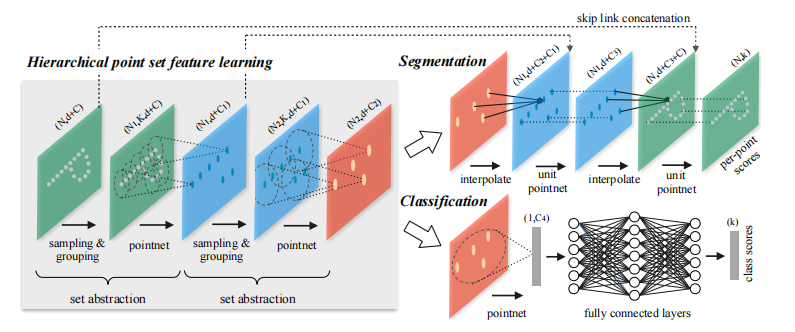
\includegraphics[scale=0.7]{doc/img/f2.png}
\caption{2}
\end{figure}
    
\end{frame}


\begin{frame}
\frametitle{采样优化策略:非均匀采样}

多尺度分组(MSG),如图(a)所示,在每一个抽象层中使用具有不同尺度的分组层,然后根据PointNets提取每个尺度的特征。不同尺度的特征被连接以形成多尺度特征。

多分辨率分组(MRG),由于上面的MSG计算开销较大,因为它在每个质心点的大规模邻域中运行PointNet。通常由于在底层时质心点的数量相当大,因此时间成本是高昂的。MRG的层特征是两个向量的拼接。一个向量(图中左侧)是通过使用单尺度分组(SSG)汇总每个子区域的特征而获得的。另一个矢量(右)是通过使用单个PointNet直接处理局部区域中的所有原始点获得的特征。当局部区域的密度低时,左侧向量比右侧向量更不可靠,因为在计算左侧向量时子区域点云稀疏导致采样不足。在这种情况下,右侧向量的权重应该更高。相反,当局部区域的密度高时,左侧矢量提供了更精细的信息,此时应该提高左侧向量的权重。

\end{frame}

\begin{frame}
\frametitle{采样优化策略:非均匀采样}


\begin{figure}
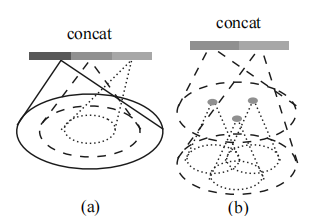
\includegraphics[scale=0.7]{doc/img/f3.png}
\caption{3}
\end{figure}
    
    
\end{frame}


\begin{frame}
\frametitle{基于点特征传播的点云分割方法}
    
使用基于特征距离的插值传播方法逆向生成前一个抽象层所有点的近邻特征,再与前一个抽象层的分组学习特征拼接为逐点分割特征,使用PointNet的部分仿射架构进行特征学习,进行下一轮特征传播,直到传播至原始点云。在插值中,使用k个最近邻的反距离加权平均特征。


$$
f^{(j)}(x)=\frac{\sum_{i=1}^{k} w_{i}(x) f_{i}^{(j)}}{\sum_{i=1}^{k} w_{i}(x)} \quad \text { where } \quad w_{i}(x)=\frac{1}{d\left(x, x_{i}\right)^{p}}, j=1, \dots, C
$$


\end{frame}
